\section{Decorrelation by Whiteninig}


% --- SLIDE 6: THE TRANSFORMATION WORKFLOW (ANIMATED) ---
\begin{frame}{Implementation Workflow (Step-by-Step)}
    \begin{columns}[c]
        % Left Column: The Steps (Text)
        \begin{column}{0.55\textwidth}
            \small
            \textbf{Standard Operating Procedure (SOP):}

            % [<+->] automatically uncovers items one by one (1, then 2, then 3...)
            \begin{enumerate}[<+->]
                \setlength\itemsep{0.5em}

                \item \textbf{Decompose:} Compute Eigen-decomposition of Covariance Matrix $\hat{\vect{\Sigma}} = \vect{P} \vect{\Lambda} \vect{P}^T$.

                \item \textbf{Transform (Whitening):} Rotate data to eliminate correlation.
                % The box appears with item 2
                \begin{equation*}
                    \boxed{\vect{Z}_i = \vect{\Lambda}^{-1/2}\vect{P}^T(\vect{x}_i - \bar{\vect{x}})}
                \end{equation*}

                \item \textbf{Estimate:} Apply simple Product Kernel on the whitened data $\vect{Z}$.

                \item \textbf{Reconstruct:} Adjust density scale to original space (Jacobian determinant).
                \[ \hat{f}_{\vect{X}}(\vect{x}) = \hat{f}_{\vect{Z}}(\vect{z}) \cdot \alert{|\hat{\vect{\Sigma}}|^{-1/2}} \]
            \end{enumerate}
        \end{column}

        % Right Column: The Image (Static)
        % We keep the image visible from the start so they can reference it while reading steps
        \begin{column}{0.45\textwidth}
            \centering
            \includegraphics[width=0.95\linewidth, height=6cm, keepaspectratio]{whitening_transform}
            \vspace{0.2em}
            \captionof{figure}{\scriptsize $\vect{X}$ (Correlated) $\to$ $\vect{Z}$ (Spherical)}
        \end{column}
    \end{columns}
\end{frame}

% --- SLIDE 6.5: MATH COMPARISON (COMPACT VERSION) ---
\begin{frame}{Conceptual Comparison: PCA vs. Whitening (1/2)}
    \small % 1. Shrink global font size slightly to prevent overflow

    % 1. THE SHARED DNA (Compacted)
    \begin{block}{The Shared DNA: Eigen-decomposition}
        \centering
        % Put equation and note on the same line to save vertical space
        $ \hat{\vect{\Sigma}} = \vect{P} \vect{\Lambda} \vect{P}^T $
        \hspace{1em}
        {\scriptsize (\textbf{P}: Rotation Matrix, \textbf{$\Lambda$}: Scale Matrix)}
    \end{block}

    \vspace{0.5em} % Minimal spacing

    % 2. THE SPLIT (Columns)
    \begin{columns}[t]
        % --- LEFT: PCA ---
        \begin{column}{0.49\textwidth}
            \onslide<2->{
                \begin{block}{1. PCA (The Rotator)}
                    \centering \footnotesize % Use smaller font inside blocks
                    \textbf{Goal:} Decorrelate (Align axes).

                    \vspace{-0.3em} % Tighten space around equation
                    $$ \vect{Y} = \underbrace{\vect{P}^T}_{\text{Rotate}} (\vect{x} - \bar{\vect{x}}) $$
                    \vspace{-0.5em}

                    \begin{itemize}
                        \setlength\itemsep{0.2em} % Tighten list items
                        \item \textbf{Shape:} Remains Elliptical.
                        \item \textbf{Variance:} Preserved ($\vect{\Lambda}$).
                        \item \textit{Not enough for Product Kernels.}
                    \end{itemize}
                \end{block}
            }
        \end{column}

        % --- RIGHT: WHITENING ---
        \begin{column}{0.49\textwidth}
            \onslide<3->{
                \begin{alertblock}{2. Whitening (The Squasher)}
                    \centering \footnotesize
                    \textbf{Goal:} Isotropy (Make Spherical).

                    \vspace{-0.3em}
                    $$ \vect{Z} = \underbrace{\alert<3>{\vect{\Lambda}^{-1/2}}}_{\text{\textbf{Scale}}} \underbrace{\vect{P}^T}_{\text{Rotate}} (\vect{x} - \bar{\vect{x}}) $$
                    \vspace{-0.5em}

                    \begin{itemize}
                        \setlength\itemsep{0.2em}
                        \item \textbf{Shape:} Becomes Spherical.
                        \item \textbf{Variance:} Normalized to 1 ($\vect{I}$).
                        \item \textit{Perfect for Product Kernels.}
                    \end{itemize}
                \end{alertblock}
            }
        \end{column}
    \end{columns}
\end{frame}


% --- SLIDE 6.6: VISUAL INTUITION (GEOMETRY) ---
\begin{frame}{Conceptual Comparison: Visual Geometry (2/2)}
    \centering
    \textbf{From Correlation to Isotropy: A Visual Journey}
    \vspace{1.5cm} % Tạo khoảng trống lớn cho hình vẽ thoáng

    % TikZ Diagram (Now bigger and clearer)
    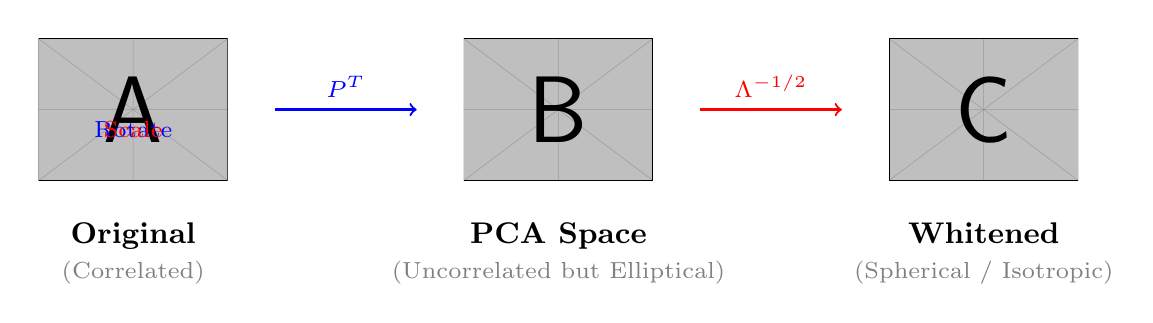
\begin{tikzpicture}[scale=1.2, transform shape]
        % STEP 1: ORIGINAL
        \node (origin) at (0,0) {\includegraphics[width=2cm]{example-image-a}}; % Placeholder: Correlated Data
        \node[below=0.2cm] at (origin.south) {\small \textbf{Original}};
        \node[below=0.6cm, gray] at (origin.south) {\scriptsize (Correlated)};

        % ARROW 1: PCA
        \draw[->, thick, blue] (1.5,0) -- (3.0,0) node[midway, above] {\scriptsize $\vect{P}^T$};
        \node[midway, below, blue] at (2.25,0) {\scriptsize Rotate};

        % STEP 2: PCA SPACE
        \onslide<2->{
            \node (pca) at (4.5,0) {\includegraphics[width=2cm]{example-image-b}}; % Placeholder: Aligned Ellipse
            \node[below=0.2cm] at (pca.south) {\small \textbf{PCA Space}};
            \node[below=0.6cm, gray] at (pca.south) {\scriptsize (Uncorrelated but Elliptical)};
        }

        % ARROW 2: WHITENING
        \onslide<3->{
            \draw[->, thick, red] (6.0,0) -- (7.5,0) node[midway, above] {\scriptsize $\vect{\Lambda}^{-1/2}$};
            \node[midway, below, red] at (6.75,0) {\scriptsize Scale};

            % STEP 3: WHITENED SPACE
            \node (white) at (9.0,0) {\includegraphics[width=2cm]{example-image-c}}; % Placeholder: Sphere
            \node[below=0.2cm] at (white.south) {\small \textbf{Whitened}};
            \node[below=0.6cm, gray] at (white.south) {\scriptsize (Spherical / Isotropic)};
        }
    \end{tikzpicture}

    \vspace{1cm}
    \onslide<3->{
        \small \textit{Note: Only the \textbf{Whitened} space is suitable for Product Kernels.}
    }
\end{frame}

% --- SLIDE 7: PERFORMANCE COMPARISON (ANIMATED) ---
\begin{frame}{Performance Comparison}

    \begin{columns}[c]
        % Left Column: Image (Always visible to set the context)
        \begin{column}{0.6\textwidth}
            \centering
            \includegraphics[height=4.0cm, keepaspectratio]{white_mkde_vs_native}
            \vspace{-0.2em}
            \captionof{figure}{\scriptsize Naive (Left) vs. Whitened (Right)}
        \end{column}

        % Right Column: Text Observations (Revealed sequentially)
        \begin{column}{0.4\textwidth}
            \small
            \textbf{Key Observations:}
            \begin{itemize}
                \setlength\itemsep{0.5em}

                % Click 2: Reveal the Failure analysis
                \item<2-> \textbf{Naive Approach:}
                \textcolor{red}{\textbf{Fail.}} Constrained to axis-aligned shapes. Misses diagonal correlations.

                % Click 3: Reveal the Success analysis
                \item<3-> \textbf{Whitened MKDE:}
                \textcolor{darkgreen}{\textbf{Success.}} Contours adapt perfectly to the data's orientation.
            \end{itemize}
        \end{column}
    \end{columns}

    \vspace{1em}

    % Click 4: Reveal the Final Verdict (The "Takeaway" message)
    \onslide<4->{
        \begin{alertblock}{Final Verdict}
            \centering \footnotesize
            Whitening enables \textbf{Product Kernels} to model complex correlations with $O(n)$ efficiency.
        \end{alertblock}
    }
\end{frame}


% --- SLIDE 5: THE MATHEMATICAL SHORTCUT (ANIMATED) ---
\begin{frame}{Generalized Estimator (Theory)}
    Instead of performing manual transformation steps, we can mathematically express the estimator directly using the **Mahalanobis Distance**:

    % 1. The Equation is always visible, but parts light up sequentially
    \begin{block}{General Multivariate KDE Equation (10.44)}
        \begin{equation}
             \hat{f}(\vect{x}) = \frac{\alert<2>{|\hat{\vect{\Sigma}}|^{-1/2}}}{nh^p} \sum_{i=1}^{n} K \left( \frac{\alert<3>{(\vect{x} - \vect{X}_i)^T \hat{\vect{\Sigma}}^{-1} (\vect{x} - \vect{X}_i)}}{h} \right)
        \end{equation}
    \end{block}

    \vspace{1em}
    % 2. Columns appear strictly when their corresponding math term is highlighted
    \begin{columns}[t]
        % Left Column: Appears on Click 2 (Matches |\Sigma|^{-1/2})
        \begin{column}{0.48\textwidth}
            \onslide<2->{
                \textbf{\alert<2>{1. Volume Correction:}}
                \begin{itemize}
                    \item The term $|\hat{\vect{\Sigma}}|^{-1/2}$ adjusts the density scale.
                    \item Ensures the total probability integrates to 1 after "stretching" space.
                \end{itemize}
            }
        \end{column}

        % Right Column: Appears on Click 3 (Matches Mahalanobis Distance)
        \begin{column}{0.48\textwidth}
            \onslide<3->{
                \textbf{\alert<3>{2. Shape Adaptation:}}
                \begin{itemize}
                    \item Uses \textbf{Mahalanobis Distance} instead of Euclidean.
                    \item Captures the correlation structure (orientation) of the data.
                \end{itemize}
            }
        \end{column}
    \end{columns}
\end{frame}

% --- SLIDE 5.0: THE LOGIC (CONCEPTUAL EVOLUTION) ---
\begin{frame}{Evolution: From Theory to Practice (1/2)}
    \small % Compact font size

    % The Narrative
    The Whitening Estimator is not a new invention. It is the \textbf{General Estimator} (Eq 10.40) where we replace the unknown parameter $\mathbf{H}$ with the \textbf{Data's Geometry} $\hat{\vect{\Sigma}}$.

    \vspace{1.5em}

    % The Logical Transformation
    \begin{columns}[c]
        % --- LEFT: GENERAL ---
        \begin{column}{0.45\textwidth}
            \begin{block}{1. General Theory}
                \centering
                We need an unknown matrix $\mathbf{H}$:
                \vspace{0.5em}
                $$ K \left( \alert<2>{\mathbf{H}^{-1}} (\vect{x} - \vect{X}_i) \right) $$
                \vspace{0.5em}
                \footnotesize \textcolor{red}{Problem:} Optimizing $\mathbf{H}$ is hard ($O(p^2)$).
            \end{block}
        \end{column}

        % --- ARROW ---
        \begin{column}{0.1\textwidth}
            \centering
            \Large \onslide<2->{$\Rightarrow$}
        \end{column}

        % --- RIGHT: WHITENING ---
        \begin{column}{0.45\textwidth}
            \begin{alertblock}{2. Whitening Practice}
                \centering
                Plug in Sample Covariance $\hat{\vect{\Sigma}}$:
                \vspace{0.5em}
                $$ K \left( \alert<2>{\hat{\mathbf{\Sigma}}^{-1}} (\vect{x} - \vect{X}_i) \right) $$
                \vspace{0.5em}
                \footnotesize \textcolor{darkgreen}{Solution:} Use data to fix orientation.
            \end{alertblock}
        \end{column}
    \end{columns}
\end{frame}

% --- SLIDE 5.1: FULL FORMULA COMPARISON (ANATOMY) ---
\begin{frame}{The "Lost Sibling" Revealed (2/2)}
    \small
    Let's compare the \textbf{General MKDE} with the \textbf{Whitening Estimator} side-by-side.
    \vspace{0.5em}

    % 1. THE GENERAL FORMULA (Reference)
    \onslide<1->{
        \textbf{1. The General Form (Eq. 10.40):}
        \begin{equation*}
            \hat{f}(\vect{x}) = \frac{1}{n \alert<2>{|\mathbf{H}|}} \sum_{i=1}^{n} K \left( \alert<3>{\mathbf{H}^{-1} (\vect{x} - \vect{X}_i)} \right)
        \end{equation*}
    }

    \vspace{1em}
    \centering \Large $\downarrow$ \normalsize \textit{Substitute $\mathbf{H} \approx \hat{\mathbf{\Sigma}}^{1/2}$ (Data-driven)}
    \vspace{1em}

    % 2. THE WHITENING FORMULA (Target)
    \onslide<1->{
        \textbf{2. The Whitening Form (Eq. 10.44):}
        \begin{equation*}
            \hat{f}(\vect{x}) = \frac{\alert<2>{|\hat{\mathbf{\Sigma}}|^{-1/2}}}{n h^p} \sum_{i=1}^{n} K \left( \alert<3>{\frac{\hat{\mathbf{\Sigma}}^{-1/2} (\vect{x} - \vect{X}_i)}{h}} \right)
        \end{equation*}
    }

    % 3. ANALYSIS BOX (Appears at the bottom)
    \vspace{0.5em}
    \begin{columns}[t]
        \begin{column}{0.48\textwidth}
            \onslide<2->{
                \begin{block}{\alert<2>{A. Volume Term}}
                    \centering \footnotesize
                    $|\mathbf{H}|$ becomes $|\hat{\mathbf{\Sigma}}|^{1/2}$. \\
                    (Normalizes the volume change).
                \end{block}
            }
        \end{column}
        \begin{column}{0.48\textwidth}
            \onslide<3->{
                \begin{block}{\alert<3>{B. Distance Term}}
                    \centering \footnotesize
                    Quadratic form becomes Mahalanobis: \\
                    $(\vect{x}-\vect{X}_i)^T \mathbf{\Sigma}^{-1} (\vect{x}-\vect{X}_i)$.
                \end{block}
            }
        \end{column}
    \end{columns}
\end{frame}

% --- SLIDE 5.2: MESSI (TRANSPARENT VERSION) ---
\begin{frame}{Intuition 1: The "Messi" Factor (Variance)}
    \footnotesize

    \begin{columns}[T]
        % --- LEFT: PROFILE (IMAGE BLENDS IN) ---
        \begin{column}{0.28\textwidth}
            \centering
            % Mẹo: Dùng chiều rộng 100% cột để ảnh to nhất có thể
            % LaTeX tự động lọc nền trong suốt của file .png
            \includegraphics[width=1.0\linewidth, keepaspectratio]{images/messi_transparent.png}

            \vspace{0.2em}
            \textbf{Scenario: La Liga}
            \begin{itemize}
                \setlength\itemsep{0em}
                \raggedright
                \item \textbf{Mean:} 5G, 10km.
                \item \textbf{A:} 5G, \textbf{12km} (Easy).
                \item \textbf{Messi:} \textbf{7G}, 10km (Hard).
            \end{itemize}
        \end{column}

        % --- RIGHT: ANALYSIS ---
        \begin{column}{0.70\textwidth}
            \begin{block}{Euclidean (Naive Fan)}
                Calculates geometric distance:
                $ d_A = \sqrt{0^2 + 2^2} = 2 \quad | \quad d_{\text{Messi}} = \sqrt{2^2 + 0^2} = 2 $

                \onslide<2->{
                    \vspace{0.2em} \textbf{\textcolor{red}{Wrong:}} "Equally impressive."
                }
            \end{block}

            \onslide<3->{
                \begin{alertblock}{Mahalanobis (The Coach)}
                    Weights by Variance ($\sigma^2$):
                    Running variance is high; Scoring variance is low.

                    \vspace{0.2em} \centering
                    \textbf{\textcolor{darkgreen}{Correct:}} Messi is the Outlier.
                \end{alertblock}
            }
        \end{column}
    \end{columns}

    % --- BOTTOM PLOT ---
    \vspace{0.5em} \centering
    \includegraphics[height=2.8cm, keepaspectratio]{images/messi_variance_plot}
\end{frame}

% --- SLIDE 5.3: CORRELATION INTUITION (ORANGE PHOTO LAYOUT) ---
\begin{frame}{Intuition 2: The "All-Rounder" Anomaly (Correlation)}
    \footnotesize

    \begin{columns}[T]
        % --- LEFT COLUMN: PROFILE CARD (30%) ---
        \begin{column}{0.28\textwidth}
            \centering
            % PHOTO HERE: Replace 'photo_orange.jpg' with your file
            \includegraphics[width=0.9\linewidth, height=2.5cm, keepaspectratio]{exs2}

            \vspace{0.5em}
            \textbf{Scenario: Idol Show}
            \begin{itemize}
                \setlength\itemsep{0em}
                \raggedright
                \item \textbf{Rule:} High Vocal $\leftrightarrow$ Avg Dance.
                \item \textbf{A (Orange):} Voc 9, Dance 6 (Normal).
                \item \textbf{B (All-Rounder):} Voc 9, Dance 9.
            \end{itemize}
        \end{column}

        % --- RIGHT COLUMN: ANALYSIS BLOCKS (70%) ---
        \begin{column}{0.70\textwidth}
            % 1. Euclidean Block
            \begin{block}{Euclidean (Blind to Context)}
                Measures straight line from Average (5,5).

                \begin{itemize}
                    \setlength\itemsep{0em}
                    \item Sees B as only "slightly" further than A.
                    \item \textbf{Fails} to see the skill trade-off pattern.
                \end{itemize}
            \end{block}

            % 2. Mahalanobis Block
            \onslide<2->{
                \begin{alertblock}{Mahalanobis (Structure Aware)}
                    Uses \textbf{Correlation Matrix} (Ellipse shape).

                    \begin{itemize}
                        \setlength\itemsep{0em}
                        \item \textbf{A (Orange):} On the ellipse edge (Expected).
                        \item \textbf{B (All-Rounder):} Far outside (The Unicorn).
                    \end{itemize}
                    \vspace{0.2em}
                    \centering \textbf{\textcolor{darkgreen}{Conclusion:}} B is a huge anomaly.
                \end{alertblock}
            }
        \end{column}
    \end{columns}

    % --- BOTTOM: THE MATH PLOT ---
    \vspace{0.5em}
    \centering
    \includegraphics[height=2.8cm, keepaspectratio]{idol_correlation_plot}
\end{frame}